
\newcommand{\geff}{\gamma_{eff}}

\section*{Общая характеристика работы}

\newcommand{\actuality}{\underline{\textbf{\actualityTXT}}}
\newcommand{\progress}{\underline{\textbf{\progressTXT}}}
\newcommand{\aim}{\underline{{\textbf\aimTXT}}}
\newcommand{\tasks}{\underline{\textbf{\tasksTXT}}}
\newcommand{\novelty}{\underline{\textbf{\noveltyTXT}}}
\newcommand{\influence}{\underline{\textbf{\influenceTXT}}}
\newcommand{\methods}{\underline{\textbf{\methodsTXT}}}
\newcommand{\defpositions}{\underline{\textbf{\defpositionsTXT}}}
\newcommand{\reliability}{\underline{\textbf{\reliabilityTXT}}}
\newcommand{\probation}{\underline{\textbf{\probationTXT}}}
\newcommand{\contribution}{\underline{\textbf{\contributionTXT}}}
\newcommand{\publications}{\underline{\textbf{\publicationsTXT}}}

Одной из альтернатив Стандартной Модели (СМ) элементарных частиц являются теории суперсимметрии 
(так называемые  SUSY-теории). Электрический дипольный момент (ЭДМ) элементарных частиц может служить
отличным инстрментом для выбора между этими двумя моделями; к примеру: в случае нейтрона, 
электрический дипольный момент, совместный со стандартной моделью, 
находится в диапазоне от $10^{-33}$ до $10^{-30}$~\ecm.~\cite{Harris:Neutron2007}, в то время как SUSY-теории
предсказывает наличие ЭДМ гораздо большей величины -- на уровне ${10^{-29} - 10^{-24}}$~\ecm. 

Поиск ЭДМ частиц был начат более 50-ти лет назад. Первый эксперимент по измерению ЭДМ нейтрона был проведён д-р. Н.Ф. Рэмзи (Dr. N.F. Ramsey) в конце 1950-х годов. По результатам эксперимента, верхняя граница ЭДМ нейтрона была ограничена величиной ${5\cdot 10^{-20}}$~\ecm.~\cite{Ramsey:Neutron1957} С тех пор было проведено множество более точных экспериментов, и на данный момент, верхняя граница на ЭДМ нейтрона находится на уровне ${2.9\cdot 10^{-26}}$~\ecm.~\cite{Baker:nEDM:Main, Baker:nEDM:Reply}

Большинство экспериментов проводятся на зарядово-неитральных частицах, таких как нейтрон или атомы. ЭДМ заряженных частиц, таких как протон или дейтрон, можно измерить в накопительном кольце, на основе прецессии поляризации пучка в электрическом поле в системе центра масс пучка.

Идея использования накопительного кольца для детектирования ЭДМ заряженный частиц появилась в процессе разработки $g-2$ эксперимента~\cite{BNL:g-2:2001} в Брукхейвенской Национальной Лаборатории (BNL, США). По результатам экспериментов в BNL, верхняя граница электрического дипольного момента мюона была установлена на уровне $10^{-19}$~\ecm.~\cite{BNL:muon_ANA:2009} В 1990-х годах, дискуссия преимущественно велась вокруг мюонного эксперимента~\cite{Farley:SREDM:Muon}, однако также рассматривался и дейтрон, у которого похожее отношение аномального магнитного момента к массе.

В 2004 году, коллаборацией srEDM (Storage Ring EDM Collaboration)~\cite{BNL:SREDM} в BNL был предложен эксперимент 970 по детектированию ЭДМ дейтрона на уровне $10^{-27}~e\cdot$см в накопительном кольце. 

Тогда же была предложена идея ``замороженного спина'' (``frozen spin'' method~\cite{Farley:SREDM:Muon}), в котором направления векторов спина и импульса (референсной) частицы совпадают в каждый момент времени. Это условие должно обеспечивать максимальный рост сигнала электрического дипольного момента при его наличии. Теретически, условие ``замороженного спина'' означает нулевой спиновый резонанс, при котором ориентация спин-вектора остается  пространственно-неизменной при отсутствии электрического дипольного момента. Тогда, любой рост вертикальной компоненты поляризациии пучка детектирует наличие электрического дипольного момента. Таким образом, измеряя  амплитуду вертикальной компоненты спина, мы определяем величину электрического дипольного момента. Реализация этой концепции потребует специальное накопительное кольцо и определенных параметров пучка.

Однако, в последствии выяснилось, что ``замороженный спин'' -- лишь одно из условий успешного детектирования электрического дипольного момента. В частности, для измерения ЭДМ с требуемой точностью необходимо накопление большой статистики, которое возможно при сохранении поляризации, то есть максимальной однонаправленности спина всех частиц в пучке, в течение достаточно длительного времени, порядка 1~000~секунд. 

Другим важным условием является требование исключения примешивания к сигналу ЭДМ сигнала магнитного дипольного момента (МДМ), возникающего из-за различного рода несовершенств элементов кольца, и соизмеримого с ЭДМ. 
Классический метод ``замороженного спина'' (когда спин-прецессия, связанная с МДМ, исключена полностью) проблематичен в этом отношении по двум причинам: 
во-первых, при приближении к состоянию ``замороженности'' спина малейшие возмущения со стороны магнитного и электрического полей приводят к нарушению ориентации оси стабильного спина, что сразу же вносит неопределенность в измерение вертикальной компоненты спина; 
во-вторых, для уменьшения скорости МДМ спин-прецессии вокруг радиальной оси до уровня, позволяющего измерить ЭДМ с точностью $10^{-29}$~\ecm, необходимо устанавливать оптические элементы ускорителя с точностью, значительно превышающей технологические возможности современных геодезических методов.

Начиная с 2005 года, на циклотроне AGOR KVI-центра передовых радиационных технологий (KVI-Center for Advanced Radiation Technology) в университете Гронингена была проведена серия тестов по технико-экономическому обоснованию эксперимента.

В 2008 году начались исследования на накопительном кольце COSY в Исследовательском центре ``Юлих'' (Forschungszentrum J\"ulich GmbH, Германия). В период с 2015 по 2019 автор принимал непосредственное участие в этих работах. Исследования велись по трем направлениям.

Первое: экспериментальное изучение декогеренции спина частиц в пучке. Поскольку кольцо COSY не отвечает требованиям реализации условия ``замороженного спина,''  декогеренция изучалась по времени исчезновения средней по пучку ассиметрии сечения взаимодействия в реакции рассеяния дейтронного пучка на углеродной мишени~\cite{COSY:SCT:IPAC15}. Вектор поляризации пучка при этом быстро прецессировал в плоскости замкнутой орбиты, что, однако, не влияет на сделанные выводы. 

Второе направление --- экспериментальное детектирование сигнала электрического дипольного момента с помощью возбуждения параметрического резонанса прецессии спина. Сила резонанса при этом пропорциональна величине детектируемого ЭДМ. Резонансный метод не требует условия ``замороженного спина,'' но его чувствительность на четыре-пять порядков ниже; в лучшем случае, его достижимый предел измерения ЭДМ находится на уровне $10^{-24}$~\ecm. 

Третье направление --- разработка метода измерения ЭДМ, и его полномасштабное моделирование с целью его совершенствования, а также  разработки новых подходов к измерению электрического дипольного момента заряженной частицы с использованием накопительного кольца.

Впоследствии, эти тесты развились в программу по изучению спин-орбитаьной динамики пучка для разработки технологий, требуемых для эксперимента по поиску ЭДМ. В этом же году было сделано второе предложение~\cite{BNL:Deuteron2008} эксперимента по поиску ЭДМ дейтрона на основе концепции ``замороженного спина''; в этот раз --- на уровне $10^{-29}$~\ecm~ при условии накопления результатов измерения в течение года.

В то же время было решено, что эксперимент по детектированию ЭДМ протона, поскольку его можно измерить в полностью электростатическом кольце, обладает некоторыми техническими достоинствами. Среди таковых предполагается возможность одновременной инжекции противоположно-циркулирующих пучков, что позволяет уменьшить систематические ошибки измерения ЭДМ протона, вызванные несовершенством элементов накопительного кольца. Тем не менее, на COSY была продолжена работа над экспериментом с дейтроном, ввиду того, что результаты, полученные для дейтрона, распространяются и на протон.

В 2011 году была сформирована коллаборация JEDI (J\"ulich Elecric Dipoe moment Investigations).~\cite{JEDI:Website} Целью коллаборации является не только разработка ключевых технологий для srEDM, но также и проведение предварительного эксперимента прямого наблюдения ЭДМ дейтрона. 

В 2018 году, JEDI-коллаборация выполнила первое измерение дейтронного ЭДМ на COSY на основе резонансного метода~\cite{COSY:Partially-Frozen-Spin, COSY:SpinTuneMapping} с использованием специально разработанного для этой цели RF Wien filter~\cite{JSlim:RFWF:Design, JSlim:RFWF:Commisioning}. В кольце с незамороженным спином 
ЭДМ генерирует мало-амплитудные осцилляции вертикакльной компоненты поляризации пучка; например, 
при импульсе дейтронов 970 МэВ/с, как на COSY, амплитуда колебаний ожидается на уровне 
$3\cdot10^{-10}$ при величине ЭДМ $d = 10^{-24}$~\ecm. В связи с малостью амплитуды колебаний, установленный в данном эксперименте предел измерения ЭДМ оценивается на уровне $d=10^{-24}$~\ecm.

% {\progress} 
% Этот раздел должен быть отдельным структурным элементом по
% ГОСТ, но он, как правило, включается в описание актуальности
% темы. Нужен он отдельным структурынм элемементом или нет ---
% смотрите другие диссертации вашего совета, скорее всего не нужен.

{\aim} данной работы является развитие метода поиска электрического дипольного момента дейтрона с использованием накопительного кольца на основе измерения частоты прецессии спина (frequency domain method) с экспериментально подтвержденной точностью.

Для~достижения поставленной цели необходимо было решить следующие {\tasks}:
\begin{enumerate}
%  \item Исследовать явление декогеренции спина пучка в окрестности нулевой спиновой частоты, а также секступольный метод её подавления. 
%  \item Исследовать влияние возмущений спиновой динамики на ЭДМ-статистику.
%  \item Исследовать влияние неточности установки E+B спин-ротаторов на систематическую ошибку ЭДМ-статистики.
%  \item Промоделировать процесс калибровки спин-тюна пучка при смене полярности ведущего поля.
	\item Формулирование метода измерения электрического дипольного момента дейтрона на основе измерения частоты прецессии спина (frequency domain method).
	\item Анализ требований к магнитооптической структуре кольца-накопителя, ориентированного на поиск электрического дипольного момента дейтрона.
	\item Исследование явления декогеренции спина пучка дейтронов в окрестности состояния ``замороженного'' спина. 
	\item Разработка метода подавления декогеренции спина с помощью нелинейных элементов.
	\item Исследование влияния различного рода несовершенств элементов кольца на спин-орбитальную динамику. 
	\item Математическое моделирование процесса калибровки нормализованной частоты прецессии спина (спин-тюн) при помеременной смене полярности ведущего поля.
	\item Анализ систематических ошибок в различных предложениях по проведению эксперимента по поиску электрического дипольного момента, и их сравнение с методом frequency domain. 
	\item Изучение накопления необходимой статистики измерения электрического дипольного момента.
\end{enumerate}

{\novelty}
\begin{enumerate}
	\item Впервые предложен метод измерения электрического дипольного момента дейтрона основанный исключительно на измерении частоты прецессии спина в накопительном кольце (frequency domain method), с оцениваемым ограничением по точности на уровне $10^{-29}$~\ecm.
	\item Изучена спин-орбитальная динамика дейтронного пучка в окрестности состояния ``замороженного'' спина в накопительном кольце для поиска электрического дипольного момента. 
	\item Предложен метод калибровки средней по пучку нормированной частоты прецессии спина, позволяющий уменьшить вклад систематических ошибок.
	\item Введено определение эффективного значения фактора Лоренца, необходимое для определения зависимости частоты прецессии спина от координат в 3-х мерном пространстве. 
	\item Сделаны статистические оценки предельной чувствительности измерения ЭДМ предложенным методом в накопительном кольце. 
%	\item Исследована систематическая ошибка эксперимента по поиску ЭДМ в накопительном кольце, связанная с бетатронными колебаниями.
	\item Проведена общая классификация методов поиска ЭДМ в накопительном кольце; систематизированы их общие проблемы.
\end{enumerate}

{\influence}. Результаты исследования вошли в Yellow Report под названием ``Feasibility Study for an EDM Storage Ring,'' подготавливаемый для CERN коллаборацией CPEDM, в которую входит коллаборация JEDI.

% здесь я пытаюсь подтянуть свои статьи по ТРИКу

Целью экспериментов по поиску ЭДМ является проверка CP-инвариантности. При этом ЭДМ элементарных частиц нарушают одновременно и P-, и T-симметрию, а следовательно требуют дополнительных модельных предположений, для того, чтобы связать их существование с CP-нарушением.~\cite[стр.~1926]{Aksentev:TRIC}

Альтернативой является эксперимент TRIC (Time Reversal Invariance at Cosy~\cite{Aksentev:TRIC}), 
в котором используется T-нечётное, P-чётное взаимодействие, а значит нарушается \emph{только} T-симметрия, 
в связи с чем никаких дополнительных предположений не требуется.
%
TRIC входит в физическую программу PAX (Polarised Antiproton eXperiments~\cite{Aksentev:PAX}), для которой требуются высокоинтенсивные поляризованные пучки. Существует два подхода к получению поляризованных пучков: спин-флиппинг и спин-филтеринг. Спин-флиппинг позволяет получать более интенсивные пучки, однако на данный момент не существует стабильно-работающих методов спин-флиппинга.

{\methods} Основными методами исследования являются математическое и компьютерное моделирование, и численный эксперимент.

{\defpositions}
\begin{enumerate}
	\item Метод измерения электрического дипольного момента дейтрона, основанный исключительно на измерении частоты прецессии спина.
	\item Принцип построения магнитооптической структуры кольца-накопителя, ориентированного на поиск электрического дипольного момента дейтрона.
	\item Результаты исследования декогеренции спина пучка дейтронов в окрестности состояния ``замороженного'' спина, и метод подавления декогеренции спина с помощью нелинейных элементов.
	\item Исследование влияния различного рода несовершенств элементов накопительного кольца 
	на спин-орбитальную динамику пучка. 
	\item Метод калибровки нормализованной частоты прецессии спина (спин-тьюн) при попеременной смене полярности ведущего поля и его численное моделирование.
	\item Результаты исследования систематических ошибок в различных предложениях по проведению эксперимента по поиску электрического дипольного момента, и их сравнение с методом Frequency Domain. 
	\item Оценка статистических свойств Frequency Domain метода измерения электрического дипольного момента 
	в накопительном кольце.
%	\item Подтверждена теория механизма секступольного подавления декогеренции. % section 2.2.7
%  	\item Подтверждено утверждение о равенстве спин-тюнов частиц с одинаковыми эффективными Лоренц-факторами; найдена интерпретация эффективного Лоренц-фактора как меры продольного эмиттанса частицы. % section 2.5.2
%  	\item Показано, что калибровка ведущего магнитного поля ускорителя посредством наблюдения частоты прецессии поляризации пучка в горизонтальной плоскости --- потенциально работающая методика.
%  	\item Доказано, что возмущения спиновой динамики пучка, вызванные бетатронными колебаниями --- пренебрежимо малый систематический эффект, поддающийся контролю в методологии частотной области. % pretty well-founded
%  % statistics
%  	\item Доказано, что эффективная длительность цикла измерения поляризации находится в диапазоне от двух до трёх постоянных времени жизни поляризации. % this is a fairly well-founded claim
%  	\item Показана принципиальная возможность получения верхнего предела оценки ЭДМ на уровне $10^{-29}~e\cdot$см за полное время измерений длительностью один год. % if beam 1e11, sampling rate 375 Hz etc
%  	\item Доказано, что угловая скорость паразитного МДМ вращения линейно зависит от среднего угла наклона спин-ротаторов, и не зависит от конкретной реализации распределения наклонов. % multiple random distributions
%  	\item Доказано, что точность установки оптических элементов ускорителя не позволяет измерять ЭДМ частицы методами пространственной области. % b/c spin precession frequency is on the order of 50 rad/sec
\end{enumerate}

{\reliability} полученных результатов обеспечивается согласованием аналитических вычислений с результатами численных экспериментов. Результаты компьютерных симуляций находятся в соответствии с результатами, полученными другими авторами, и результатами, полученными в экспериментах на ускорителе COSY (Исследовательский центр ``Юлих,'' Германия).


{\probation}
Основные результаты работы докладывались~на:
\begin{itemize}
\item IIX международной концеренции по ускорителям заряженных частиц IPAC'17, Копенгаген, Дания.
\item X международной конференции по ускорителям заряженных частиц IPAC'19, Мельбурн, Австралия.
\item конференциях коллаборации JEDI, Юлих, Германия, 2017--2019.
\item III международной конференции ``Лазерные, плазменные исследования и технологии,'' (LaPlas) Москва, Россия. 
\item IV междунарожной конференции LaPlas, Москва, Россия.
\item V международной конференции LaPlas, Москва, Россия.
\item студенческих семинарах Института Ядерных Исследований, Исследовательский Центр ``Юлих,'' Германия.
\end{itemize}

{\contribution} Все положения, выносимые на защиту, получены автором лично. Результаты аналитического и численного исследования спин-орбитальной динамики пучка для моделирования метода измерения электрического дипольного момента дейтрона с помощью измерения прецессии спина в накопительном кольце получены автором лично либо при участии научного руководителя. Вклад соавторов в результаты, полученные совместно, оговаривается в тексте диссертации для каждого случая.
%Автор принимал активное участие в коллаборации JEDI, а также подготовке Yellow Report для CERN.

%\publications\ Основные результаты по теме диссертации изложены в ХХ печатных изданиях~\cite{Sokolov,Gaidaenko,Lermontov,Management},
%Х из которых изданы в журналах, рекомендованных ВАК~\cite{Sokolov,Gaidaenko}, 
%ХХ --- в тезисах докладов~\cite{Lermontov,Management}.

\ifnumequal{\value{bibliosel}}{0}{% Встроенная реализация с загрузкой файла через движок bibtex8
    \publications\ Основные результаты по теме диссертации изложены в 7 печатных изданиях, 
    \hl{X из которых изданы в журналах}, рекомендованных ВАК, 
    7 "--- в тезисах докладов.%
}{% Реализация пакетом biblatex через движок biber
%Сделана отдельная секция, чтобы не отображались в списке цитированных материалов
    \begin{refsection}[vak,papers,conf]% Подсчет и нумерация авторских работ. Засчитываются только те, которые были прописаны внутри \nocite{}.
        %Чтобы сменить порядок разделов в сгрупированном списке литературы необходимо перетасовать следующие три строчки, а также команды в разделе \newcommand*{\insertbiblioauthorgrouped} в файле biblio/biblatex.tex
        \printbibliography[heading=countauthorvak, env=countauthorvak, keyword=biblioauthorvak, section=1]%
        \printbibliography[heading=countauthornotvak, env=countauthornotvak, keyword=biblioauthornotvak, section=1]%
        \printbibliography[heading=countauthorconf, env=countauthorconf, keyword=biblioauthorconf, section=1]%
        \printbibliography[heading=countauthor, env=countauthor, keyword=biblioauthor, section=1]%
        \nocite{%Порядок перечисления в этом блоке определяет порядок вывода в списке публикаций автора
	        	TRIC,% VAK, Scopus, WoS
	        	PAX,% Scopus, WoS
	        	Stats,% Scopus, WoS
	        	Modeling, % Scopus, WoS
                Aksentev:IPAC17,% Scopus
                Aksentev:LaPlas17,Aksentev:LaPlas18,Aksentev:LaPlas19,% РИНЦ
                Aksentev:IPAC19:GFF,Aksentev:IPAC19:SMP,Aksentev:IPAC19:DECOH% Scopus
        }%
        \publications\ Основные результаты по теме диссертации изложены в~\arabic{citeauthor}~печатных изданиях:
        \arabic{citeauthornotvak} изданы в журналах, индексируемых в международных базах цитирования Scopus и Web of Science,
        %из которых \arabic{citeauthorvak} в журнале, рекомендованном ВАК, 
        а \arabic{citeauthorconf} "--- в~трудах докладов на международных конференциях. Из последних, 4 работы входят в базу Scopus, 3 в РИНЦ.
    \end{refsection}
    \begin{refsection}[vak,papers,conf]%Блок, позволяющий отобрать из всех работ автора наиболее значимые, и только их вывести в автореферате, но считать в блоке выше общее число работ
        \printbibliography[heading=countauthorvak, env=countauthorvak, keyword=biblioauthorvak, section=2]%
        \printbibliography[heading=countauthornotvak, env=countauthornotvak, keyword=biblioauthornotvak, section=2]%
        \printbibliography[heading=countauthorconf, env=countauthorconf, keyword=biblioauthorconf, section=2]%
        \printbibliography[heading=countauthor, env=countauthor, keyword=biblioauthor, section=2]%
        \nocite{TRIC}%vak
        \nocite{Stats, PAX, Modeling}%notvak
        \nocite{Aksentev:LaPlas17,Aksentev:LaPlas18,Aksentev:LaPlas19,Aksentev:IPAC17,%
	        	Aksentev:IPAC19:GFF,Aksentev:IPAC19:SMP,Aksentev:IPAC19:DECOH}%conf
    \end{refsection}
}
%При использовании пакета \verb!biblatex! для автоматического подсчёта
%количества публикаций автора по теме диссертации, необходимо
%их~здесь перечислить с использованием команды \verb!\nocite!.
 % Сеничев сказал упростить введение для автореферата
% Характеристика работы по структуре во введении и в автореферате не отличается (ГОСТ Р 7.0.11, пункты 5.3.1 и 9.2.1), потому её загружаем из одного и того же внешнего файла, предварительно задав форму выделения некоторым параметрам

%Диссертационная работа была выполнена при поддержке грантов ...

%\underline{\textbf{Объем и структура работы.}} Диссертация состоит из~введения,
%четырех глав, заключения и~приложения. Полный объем диссертации
%\textbf{ХХХ}~страниц текста с~\textbf{ХХ}~рисунками и~5~таблицами. Список
%литературы содержит \textbf{ХХX}~наименование.

\section*{Содержание работы}
Во \underline{\textbf{введении}} обосновывается актуальность
исследований, проводимых в~рамках данной диссертационной работы,
приводится обзор научной литературы по изучаемой проблеме,
формулируется цель, ставятся задачи работы, излагается научная новизна
и практическая значимость представляемой работы.

% Здесь можно расписать поподробнее, потому что большинство людей не будут
% читать сам диссер, а ознакомятся только с авторефератом
\usepgfplotslibrary{fillbetween}

\textbf{Глава 1} посвящена анализу методологии измерения электрического дипольного момента (ЭДМ) 
элементарой частицы при помощи накопительного кольца, работающего в режиме ``замороженного спина.'' 

Понятие ``замороженный спин'' определено как состояние, при котором
направление спин-вектора частицы зафиксировано относительно её вектора импульса; 
отмечено преимущество работы в режиме ``замороженного спина,'' а также условия его реализации 
в накопительных кольцах различных типов (чисто электростатические, чисто магнитные, комбинированные).

Проводится анализ двух магистральных подходов к измерению ЭДМ частицы в накопительном кольце
с замороженным спином (измерения, основанные на наблюдении набега фазы~\cite{BNL:Deuteron2008}, 
или частоты~\cite{Koop:SpinWheel2015} колебаний вектора поляризации пучка), 
с целью формулирования критериев успешности методики измерений. 

Систематизируются основные проблемы, возникающие при попытке измерить ЭДМ частицы 
в накопительном кольце при любом из существующих подходов:
\begin{enumerate*}[(1)]
	\item возмущения спиновой динамики частиц;\label{itm:prob-smp}
	\item спин-декогеренция;\label{itm:prob-sdecoh}
	\item неидеальности оптической структуры ускорителя (вызывает ложный сигнал ЭДМ).\label{itm:prob-imp}
\end{enumerate*}

Описывается метод (Frequency Domain Method), разработанный с целью решения 
всех поставленных выше проблем. Главными особенностями метода являются:
\begin{enumerate}[(1)]
	\item Величина ЭДМ вычисляется из измерений совокупной (МДМ+ЭДМ) частоты спин-прецессии.
	\item Для стабилизации оси стабильного спина частицы используется собственная 
	(связанная с неидеальностями оптической структуры) частота МДМ спин-прецесии ускорителя.
	\item МДМ компонента частоты спин-прецессии устраняется в конечной статистике путём сравнения 
	совокупных частот в циклах с противоположным направлением движения пучка.
\end{enumerate}

Представлены три варианта магнитооптической структуры накопительного кольца 
для измерения ЭДМ дейтрона предлагаемым методом: 
в структуре с ``замороженным спином'' (FS, Рис.~\ref{fig:lattices:FS})
горизонтальные проекции спин-вектора и вектора импульса частицы 
сонаправлены \emph{в каждый момент времени});
в двух структурах,  реализующих состояние ``квази-замороженного спина'' (QFS), условие
``замороженности'' выполняется \emph{в среднем}. 

\begin{figure}[H]\centering
	\begin{minipage}{.5\linewidth}
	\subbottom[FS-структура\label{fig:lattices:FS}]{%
		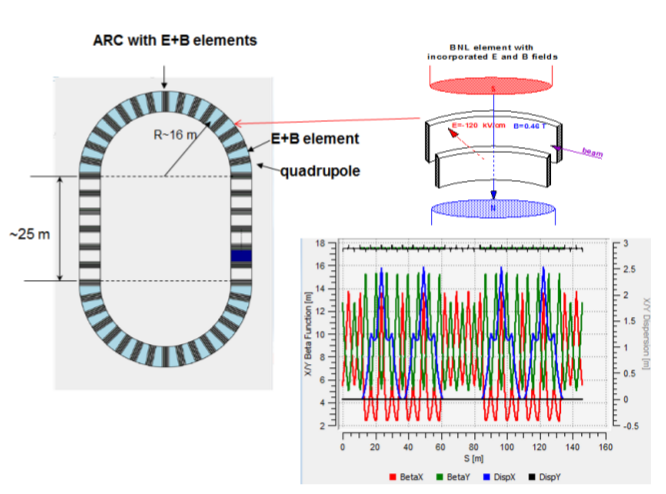
\includegraphics[height=.2\paperheight]{images/chapter2/BNL_lattice}}
	\end{minipage}%
	\begin{minipage}{.5\linewidth}
	\subbottom[{QFS-структура с пространственно-разделёнными\newline E- и B-полями\label{fig:lattices:6_3}}]{%
		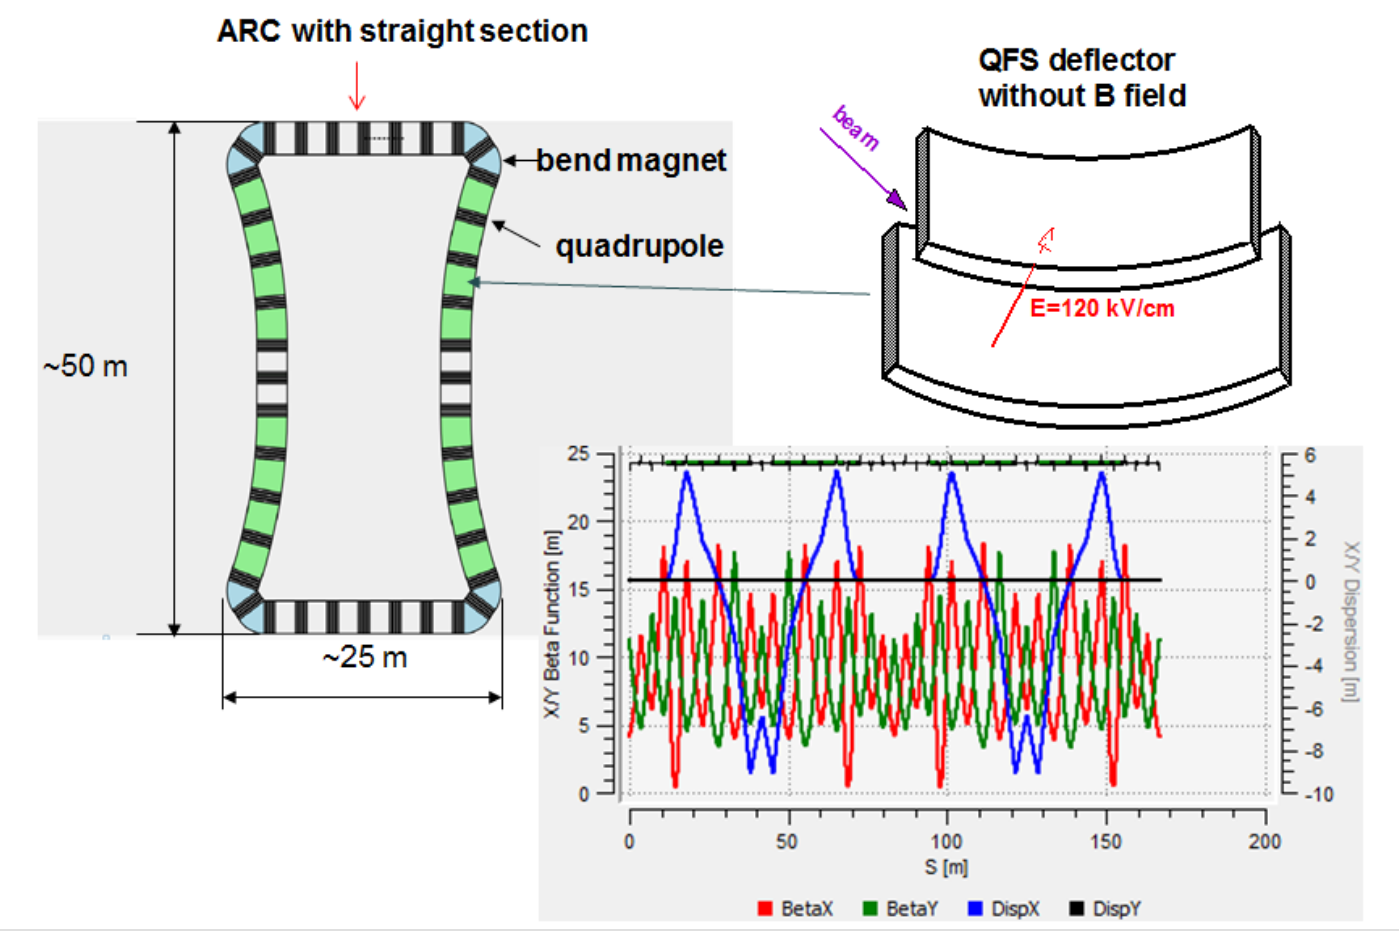
\includegraphics[height=.2\paperheight, trim=0 3 0 0, clip]{images/chapter2/6_3_lattice}}
	\end{minipage}
	\begin{minipage}{.5\linewidth}{
	\subbottom[{QFS-структура с пространственно-совмещёнными\newline E- и B-полями\label{fig:lattices:E+B}}]{%
		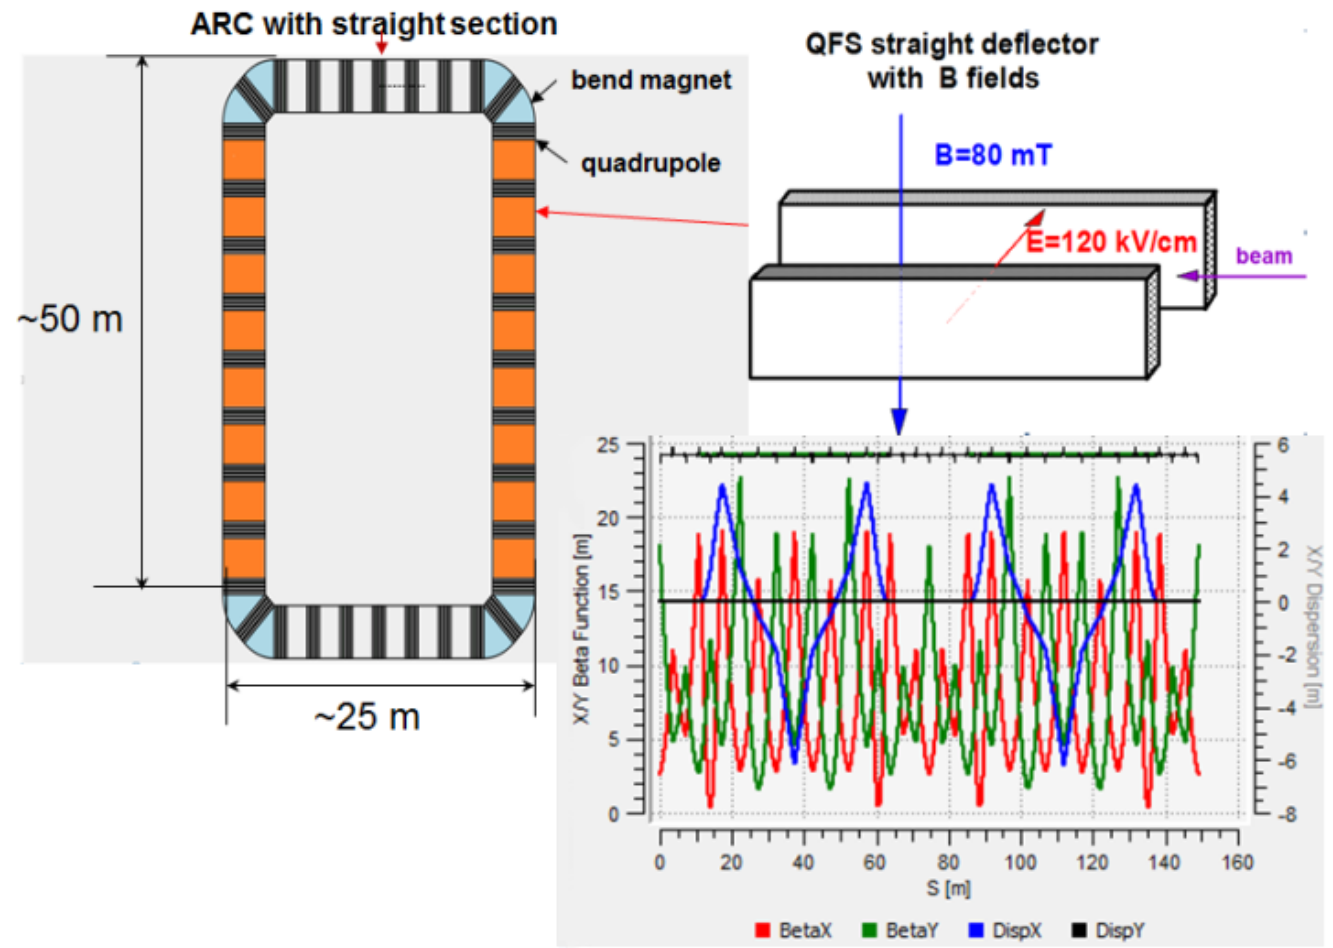
\includegraphics[height=.2\paperheight]{images/chapter2/E+B_lattice}}}
	\end{minipage}%
	\begin{minipage}{.5\linewidth}\captionsetup{width=.85\linewidth}
	\caption{Варианты магнитооптических структур для поиска ЭДМ в накопительном кольце}
	\end{minipage}
\end{figure}

Преимущество кольца QFS-типа состоит в относительной простоте исполнения: 
в предложенных вариантах используются либо
\begin{enumerate*}[(\bfseries i\normalfont)]
	\item цилиндрические электростатические дефлекторы и магнитные диполи раздельно
	 (Рис.~\ref{fig:lattices:6_3}), либо
	\item прямые фильтры Вина (Рис.~\ref{fig:lattices:E+B}).	
\end{enumerate*}
Простота исполнения, в свою очередь, позволяет использовать QFS структуру в неспециализированном под
измерения ЭДМ накопительном кольце.

\textbf{Глава 2} посвящена анализу проблем измерения ЭДМ частицы 
в накопительном кольце с замороженным спином и поиску их решений. 

Рассматриваются следующие проблемы:

\textbf{Возмущения спиновой динамики частицы,} вызванные её бетатронными колебаниями, и их влияние на ЭДМ-статистику частотного метода измерений.
%
Суть проблемы состоит в возможном несоответствии между данными поляриметрии и фитируемой к модели, 
возникающем из-за вариации направления осей стабильного спина частиц пучка, 
вовлечённых в бетатронное движение.

Решение уравнения спин-динамики (уравнение Томаса-Баргманна-Мишеля-Телегди)
для вертикальной компоненты спин-вектора:
\begin{align}
s_y &= a\cdot \sin(\omega\cdot t + \phi)\notag\\
	  &= \sqrt{\bkt{\bar n_y\bar n_z}^2 + \bar n_x^2} \cdot \sin\bkt{2\pi\cdot\nu_s\cdot \frac{t}{T} + \phi},
\end{align}
где $\nu_s$ это спин-тюн частицы, $T$ её период обращения в кольце, а $\nbar$ -- ось стабильного спина, \emph{меняющая своё направление} во время бетатронного движения.~\cite[стр.~11]{Shatunov} В связи с этим, фитирование данных гармонической моделью с постоянными
параметрами составляет систематическую ошибку спецификации регрессионной модели.

На сколько вариация в амплитуды колебаний вертикальной
компоненты поляризации влияет на систематическую ошибку оценки частоты колебаний -- 
и был интересовавший нас вопрос.

Основные выводы, сделанные на основе анализа данных моделирования, таковы:
\begin{enumerate}
	\item Осцилляции амплитуды сигнала очень малы. Они происходят на уровне не более $10^{-4}$ (при
	распределении углов наклона элементов ${N(0, 3\cdot 10^{-2})}$ градусов), 
	тогда как ожидаемая неточность измерений поляризации находится 	на уровне единиц процентов. 
	Это значит, что суперпозиция систематической ошибки и случайной ошибки измерения
	не будет проявлять статистически-значимую систематичность.
	\item Коэффициент корреляции между оценками амплитуды $\hat a$ и частоты $\hat\omega$ не значителен. Колебания амплитуды
	влияют на оценку $\hat a$ в первую очередь; их влияние на оценку $\hat\w$ опосредован, и описывается
	коэффициентом корреляции. Так как он меньше 10\%, даже если колебания окажутся достаточными, 
	чтобы повлиять на оценку амплитуды, их влияние на оценку частоты будет уменьшен по крайней мере в 10 раз.
	\item Этот систематический эффект контролируется, что является основным достоинством методологий
	частотной области. Вводя в систему внешнее магнитное поле	колебания $\bar n$ могут быть 
	непрерывно минимизированы  до необходимого уровня без каких-либо модификаций паттерна эксперимента.
\end{enumerate}

\textbf{Декогеренция спинов} частиц продольно-поляризованного пучка 
при работе в режиме замороженного спина.

Проблема спин-декогеренции пучка вызвана различием частот прецессии спинов частиц пучка 
при движении в ускорителе, что в свою очередь связано с разницей равновесных уровней энергии частиц. 

Для решения проблемы спин-декогеренции применяют~\cite{COSY:SCT:IPAC15, COSY:SCT:1000sec} 
нелинейные элементы (секступоли), влияющие одновременно на длины орбит бетатрон-осциллирующих частиц  
и на коэффициент сжатия орбиты ${\alpha = \alpha_0 + \alpha_1\delta}$ (где ${\delta=\Delta p/p_0}$).

Была разработана численная модель секступольного метода подавления спин-декогеренции 
в идеально отъюстированном (т.е. отсутствует МДМ спин-прецессия вокруг радиальной оси) накопительном кольце 
FS-типа (Рис.~\ref{fig:lattices:FS}). В результате моделирования были получены данные, представленные на Рис.~\ref{fig:decoh:perfect}. Как следует из рисунка, при включении секступольных полей теряется зависимость
нормированной частоты прецессии спина частицы (спин-тюна) от её координаты в поперечной к оптической оси
 плоскости ($x$--$y$) и от её энергии $\delta = \Delta K/K_0$ 
 (где $K$ -- кинетическая энергия частицы, индекс 0 обозначает референсную частицу).

\begin{figure}[H]
	\centering
	\begin{minipage}{.5\linewidth}
	\subbottom[В горизонтальном направлении]{%
		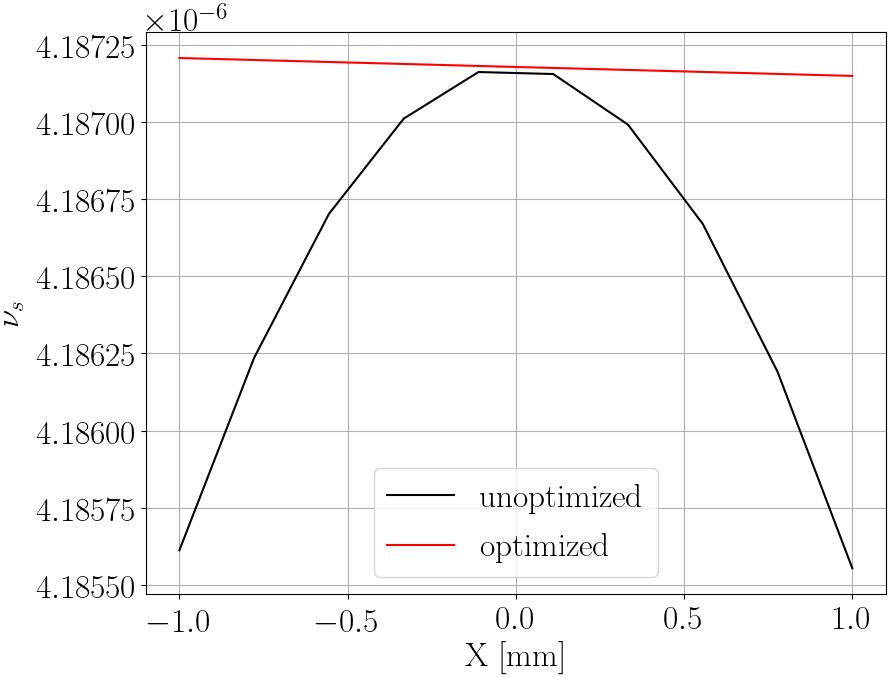
\includegraphics[height=.2\paperheight]{images/decoh_sim/spin_tune_decoh_x_offset}}
	\end{minipage}%
	\begin{minipage}{.5\linewidth}
	\subbottom[В вертикальном направлении]{%
		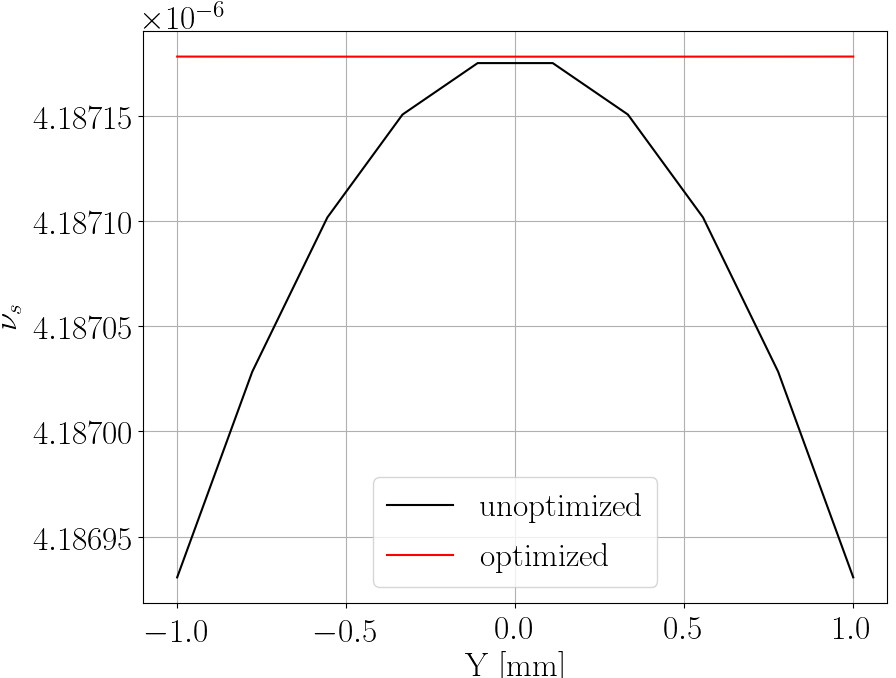
\includegraphics[height=.2\paperheight]{images/decoh_sim/spin_tune_decoh_y_offset}}
	\end{minipage}
	\begin{minipage}{.5\linewidth}
	\subbottom[По энергии]{%
		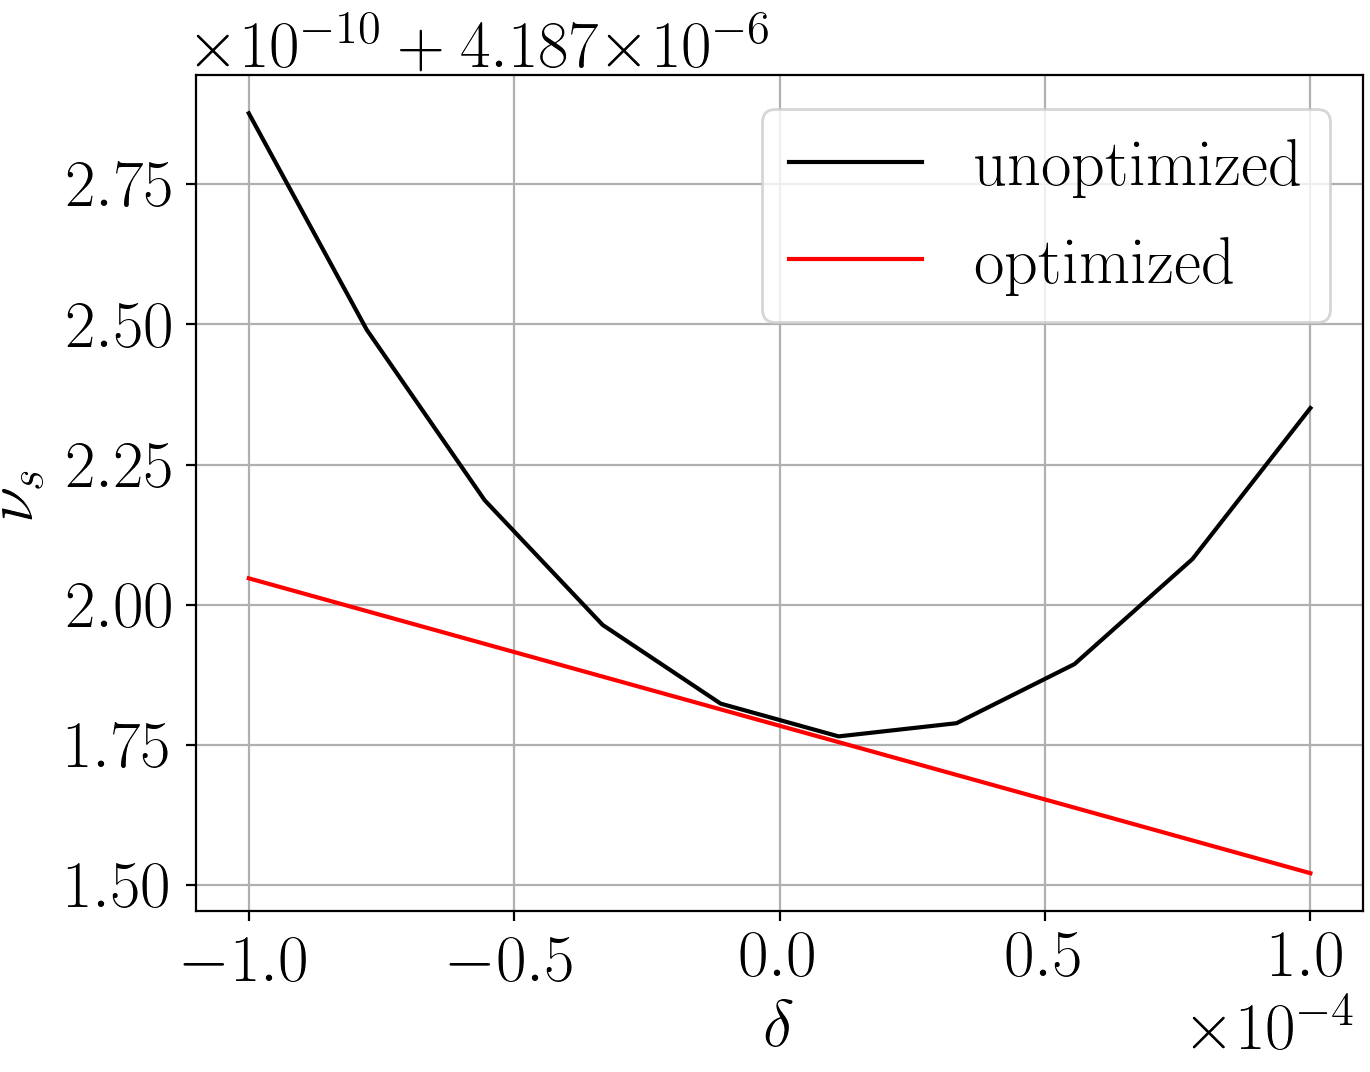
\includegraphics[height=.2\paperheight]{images/decoh_sim/spin_tune_decoh_d_offset_1}}
	\end{minipage}%
	\begin{minipage}{.5\linewidth}
	\caption{Зависимость спин-тюна частицы от её смещения от референсной частицы.\label{fig:decoh:perfect}
	Цветом выделены зависимости при нулевом (чёрный) и оптимизированном (красный) значениях градиента секступоля}
	\end{minipage}
\end{figure}

В подразделе 2.2.6 описаны результаты численного моделирования секступольного метода 
подавления спин-декогеренции в \emph{неидеальном} ускорителе; 
на основе результатов моделирования был проанализирован
эффект секступольных полей на спин-тюн частицы, а также и на направление оси стабильного спина этой частицы. 
По результатам анализа был сделан важный вывод: секступольные поля выравнивают не только спин-тюны
частиц, но и направления их осей стабильного спина (см. Рис.~\ref{decoh:fig:nbar_vs_ST}).

\begin{figure}[H]\centering
	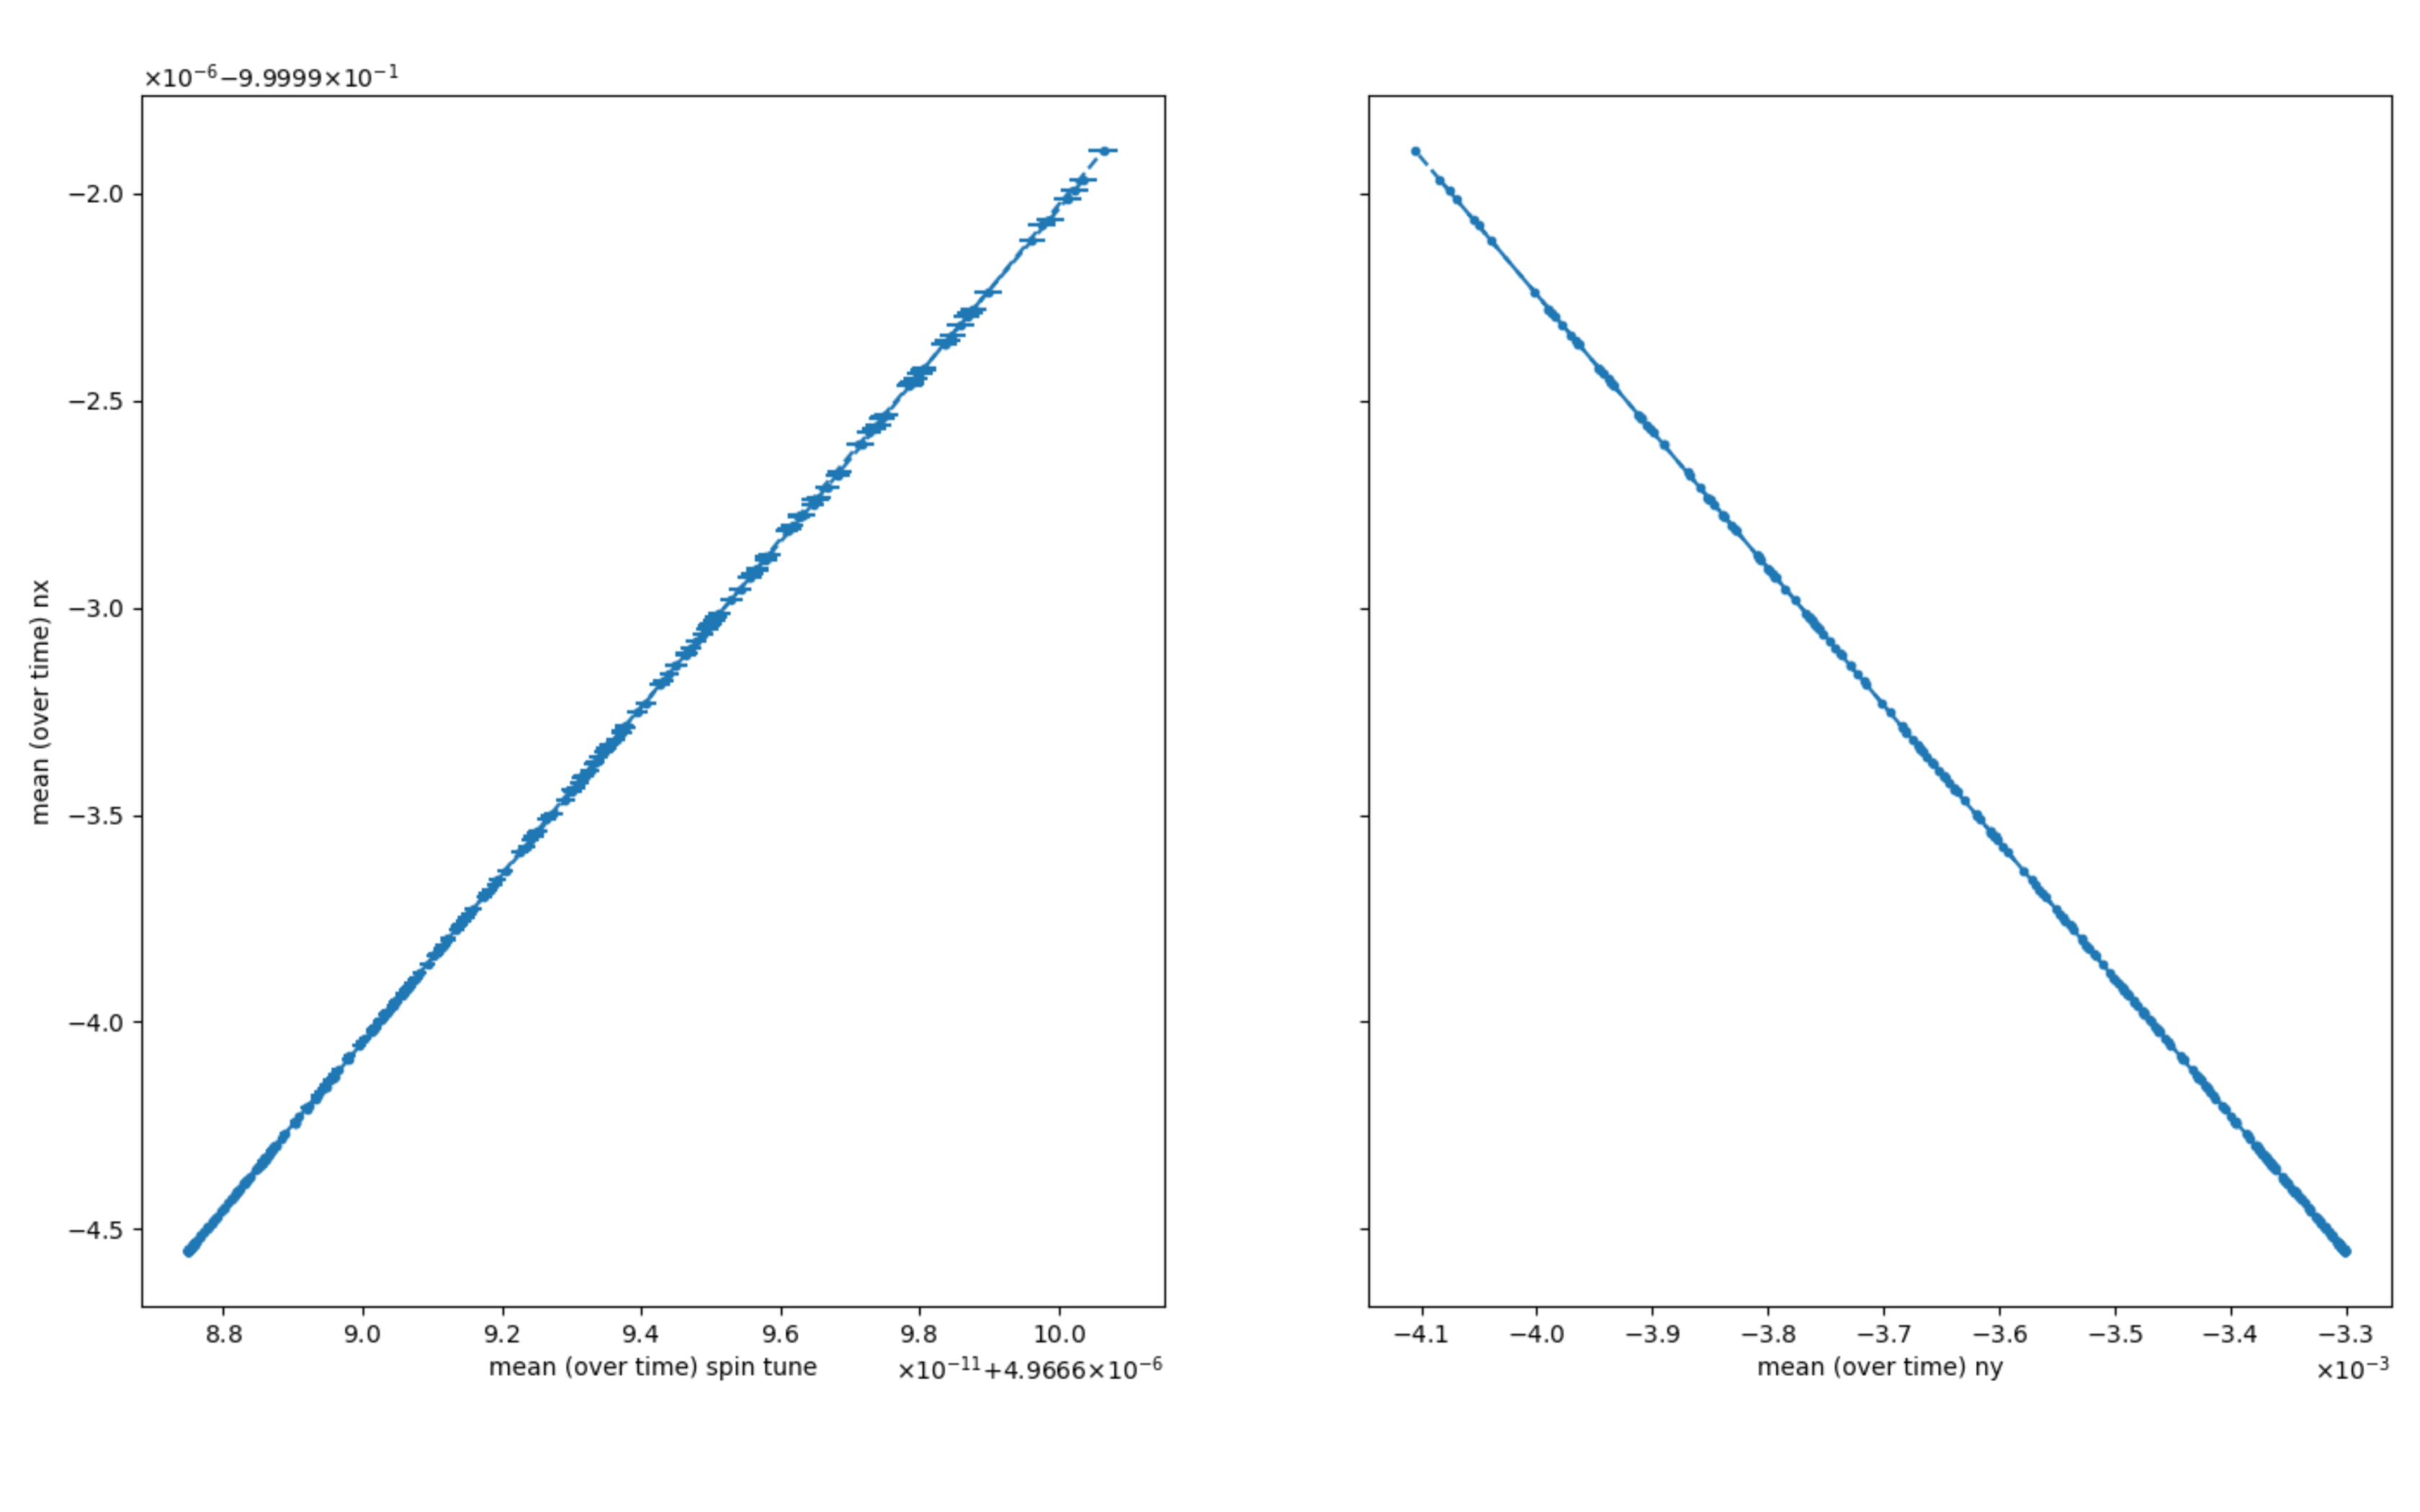
\includegraphics[height=.3\paperheight]{images/decoh_sim/mean_n_bar_vs_spin_tune}
	\caption{Средние уровни поперечных компонент осей стабильного спина частиц, в зависимости от уровня их спин-тюна\label{decoh:fig:nbar_vs_ST}}
\end{figure}

Как было отмечено ранее, секступольное поле влияет на декогеренцию двумя путями: 
модифицируя 
\begin{enumerate*}[(1)] 
	\item коэффициент сжатия орбиты и 
	\item длину орбиты частицы.
\end{enumerate*}
В подразделе 2.2.7 анализируется, каким образом каждый из обозначенных механизмов 
подавления спин-декогеренции отражается на зависимости спин-тюна частицы
от её равновесного уровня энергии.

Свойства \textbf{МДМ компоненты частоты спин-прецессии вокруг радиальной оси} $\W_x^{MDM}$, вызванной 
неидеальностями оптической структуры ускорителя, и составляющей основную 
систематическую ошибку измерений ЭДМ в накопительном кольце (любым из методов), анализируются в разделе 2.3.

В подразделе 2.3.1 подтверждаются следующие свойства $\W_x^{MDM}$ (см. Рис.~\ref{fig:syst:linearity}):
\begin{enumerate*}[(1)]
	\item зависимость $\W_x^{MDM}$ \emph{только} от среднего угла наклона спин-ротаторов $\avg{\Theta_{tilt}}$, 
	но \emph{не} от конкретной последовательности наклонов элементов $\{\Theta_{tilt}^{(i)}\}_{i\in J}$;
	\item зависимость $\W_x^{MDM}(\avg{\Theta_{tilt}}) = L(\avg{\Theta_{tilt}})$ носит линейный характер.
\end{enumerate*}

В подразделе 2.3.2 величина $\W_x^{MDM}$ сравнивается для двух противоположных направлений движения пучка:
по (CW) и против (CCW) часовой стрелки. Результаты моделирования представлены на Рис.~\ref{fig:syst:asym}.
\begin{figure}[H]\centering
	\subbottom[]{%
		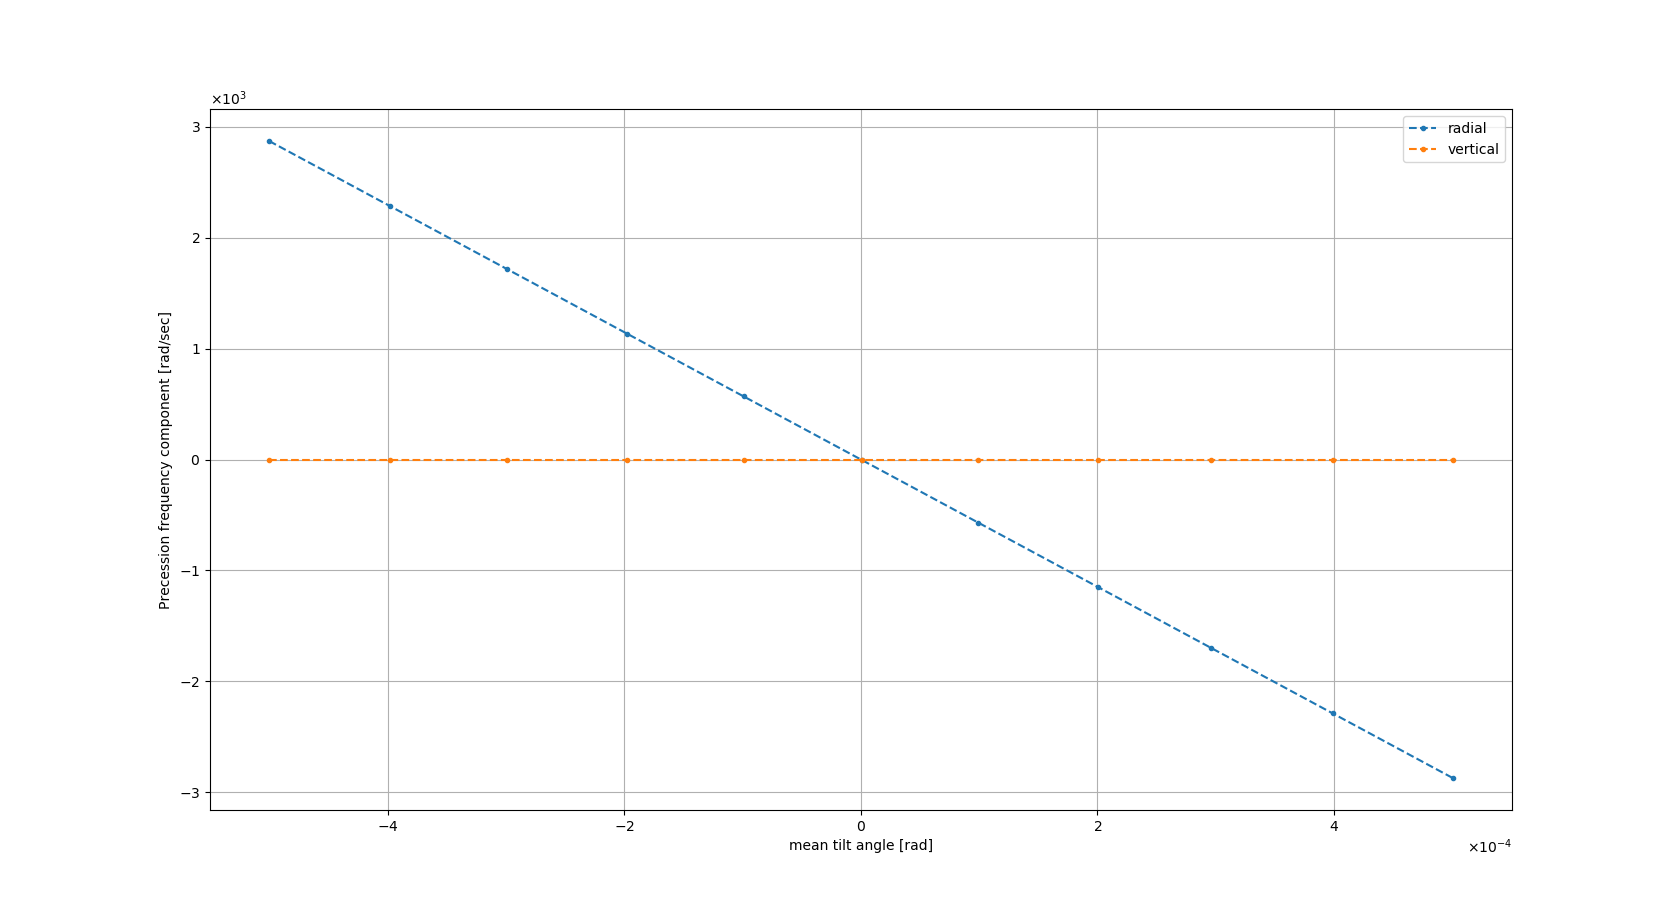
\includegraphics[height=.2\paperheight]{images/fake_signal_sim/linearity_test_shifting_gauss_freq}
	}
	\subbottom[]{%
		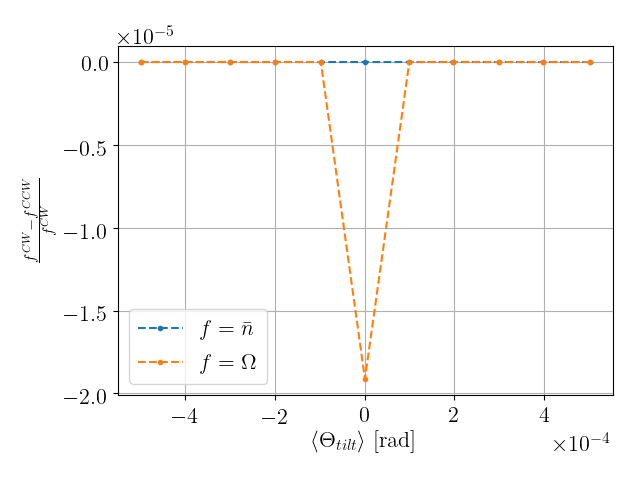
\includegraphics[height=.2\paperheight]{images/fake_signal_sim/linearity_test_shifting_gauss_rel_diff}	
	}
	\caption{Результаты исследования свойств частоты МДМ спин-прецессии в неидеальном ускорителе:
		(а) зависимость компонент частоты МДМ спин-прецессии $\vec\W^{MDM}$ референсной частицы 
		в неидеальной FS-структуре~\ref{fig:lattices:FS} 
		cо случайно-распределёнными ошибками установки спин-ротаторов
		от их среднего угла наклона $\avg{\Theta_{tilt}}$\label{fig:syst:linearity};
		(б) относительная разница между радиальными компонентами оси стабильного спина и угловой скоростью поворота спина, посчитанная относительно значения для CW-циркулирующего пучка\label{fig:syst:asym}
	}
\end{figure}

По результатам моделирования сделан вывод о том, что при движении пучка в любом из направлений 
ось стабильного спина $\nbar$ наклонена одинаково; при этом существует \emph{различие} 
между спин-тюнами CW и CCW пучков, но на уровне не более десятых долей процента, 
которое тем сильнее, чем меньше модуль $\W_x^{MDM}$. 
Эта \emph{разница}  свидетельствует об асимметричности ускорительной структуры 
относительно обращения направления движения, с точки зрения спиновой динамики, 
и может объясняться различием референсных орбит CW и CCW пучков. 

Проблема \textbf{смены полярности ведущего поля ускорителя} рассмотрена в разделе 2.4. 
Эта процедура необходима для смены направления движения дейтронного пучка в ускорителе, 
т.е. для сокращения в конечном выражении оценки ЭДМ МДМ компоненты совокупной частоты прецессии, 
измеряемой в методах частотной области:
\begin{align*}
\hat\W_{EDM} &= \frac12\left[\hat\W_{net}^+ + \hat\W_{net}^-\right], \\
\W_{net}^\pm  &= \W_{EDM} \pm \W_{MDM}.
\end{align*}

Необходимо отметить, что целью смены полярности ведущего поля является 
точное воспроизведение радиальной компоненты частоты МДМ прецессии $\W_x^{MDM}$, 
индуцированной полями неидеальности оптической структуры ускорителя. 
Этот момент часто упускается из виду: простого воспроизведения величины \emph{магнитного поля} 
не достаточно, поскольку точка инжекции центра масс пучка, а значит его длина орбиты --- 
и, соответственно, спин-тюн --- подвержена вариации. (Не говоря о возможной асимметричности 
оптической структуры кольца относительно обращения направления движения пучка, 
с точки зрения спиновой динамики.) Таким образом, необходимо восстанавливать не величину поля, 
а эффективный Лоренц-фактор центра масс пучка.

Для калибровки эффективного Лоренц-фактора в \emph{FD}-методе измеряется вертикальная компонента
ЭДМ+МДМ частоты спин-прецессии $\W_y$; пучок при этом выводится из состояния ``замороженного спина.'' 

В результате моделирования, были получены результаты, представленные на Рис.~\ref{fig:calib}.
%
Можно видеть, что при уменьшении разницы ${\Delta\W_y^{MDM} < 10^{-7}}$~рад/сек 
(точность определения частоты, достигаемая при фитировании данных одного цикла), 
разница ${\Delta \W_x^{MDM} < 10^{-8}}$~рад/сек (т.е. на порядок меньше статистической погрешности). 
Это говорит о принципиальной возможности использования частоты прецессии спина в горизонтальной плоскости 
для калибровки частоты прецессии в вертикальной плоскости.

\begin{figure}[H]\centering
	\begin{minipage}{.5\linewidth}
	\subbottom[]{%
		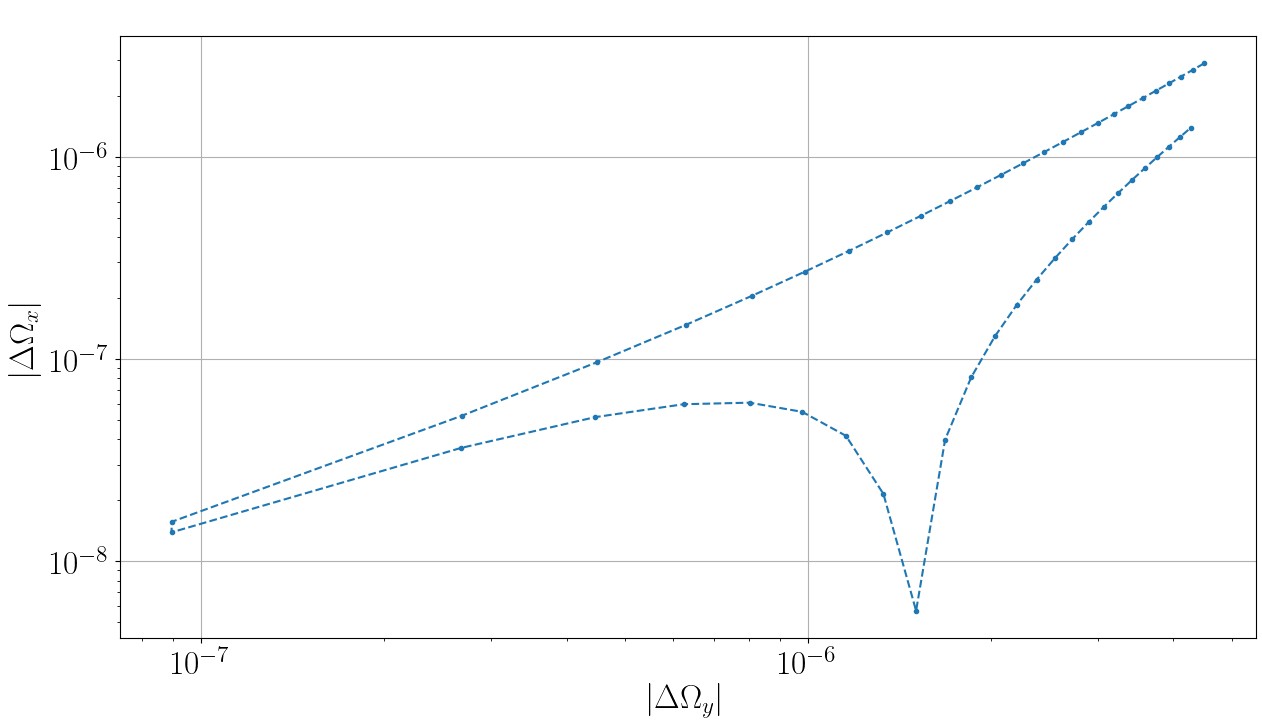
\includegraphics[height=.15\paperheight]{images/GFF/GFF_omegas_range_X}}
	
	\end{minipage}%
	\begin{minipage}{.5\linewidth}
	\subbottom[]{%
		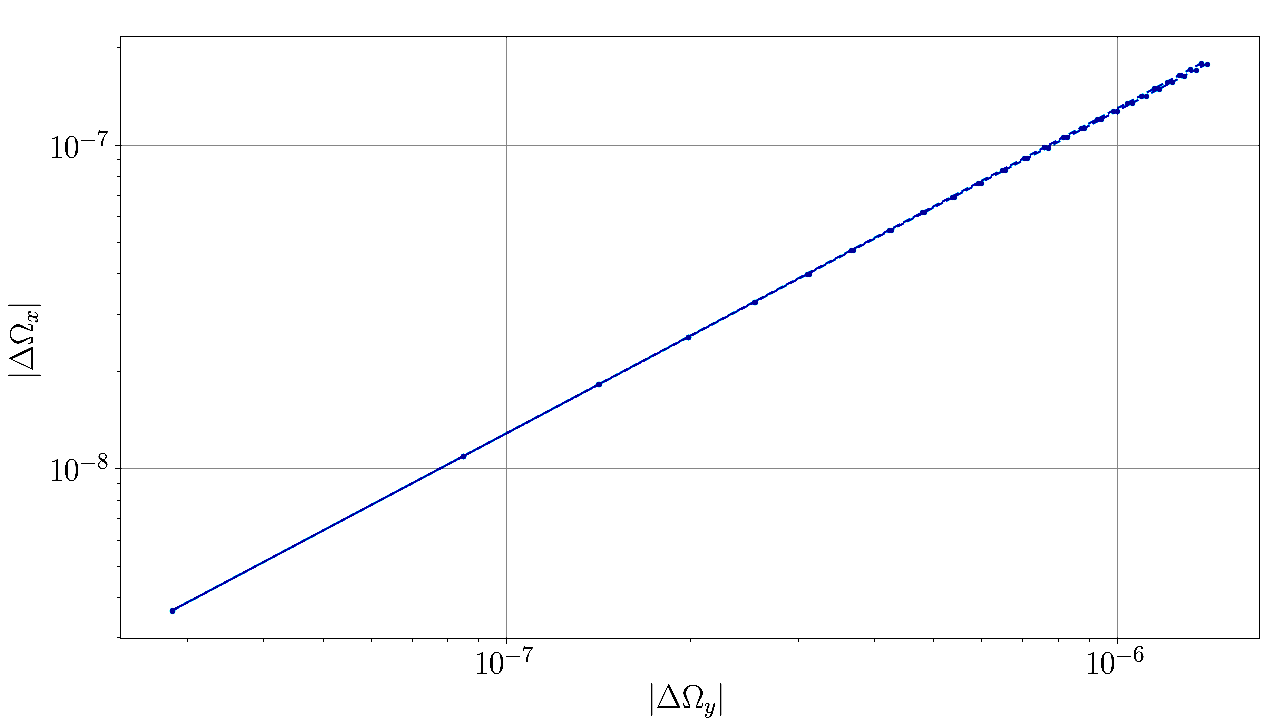
\includegraphics[height=.15\paperheight]{images/GFF/GFF_omegas_range_Y}}
	\end{minipage}
	\begin{minipage}{.5\linewidth}
	\subbottom[]{%
		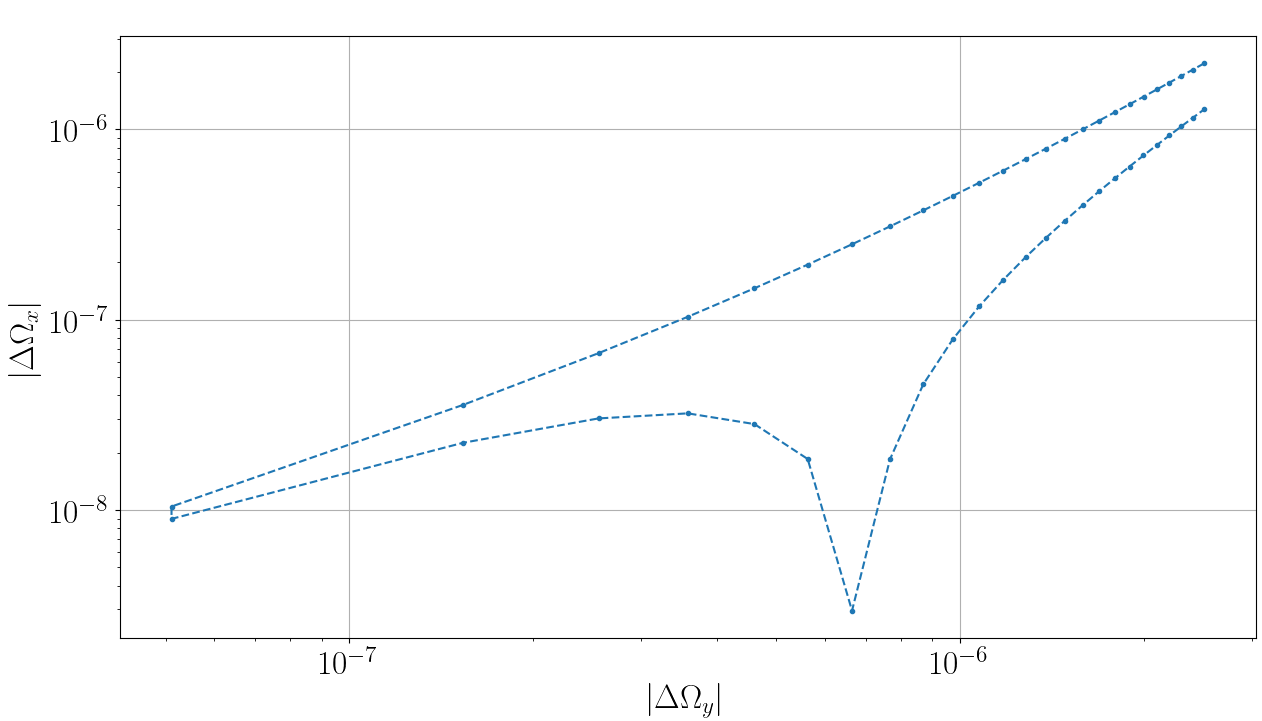
\includegraphics[height=.15\paperheight]{images/GFF/GFF_omegas_range_D}}
	\end{minipage}%
	\begin{minipage}{.5\linewidth}
	\caption{Разница между радиальными компонентами частоты прецессии CW и CCW пучков
		в зависимости от разницы вертикальных компонент (калибровочный график).\label{fig:calib}
		Рассмотрены случаи спин0декогеренции, вызванной:
	(а) бетатронным движением в горизонтальной плоскости; 
	(б) бетатронным движением в вертикальной плоскости;
	(в) синхротронным движением.
	}
	\end{minipage}
\end{figure}

Отдельно в разделе 2.5 рассматривается вопрос интерпретации введённого в подразделе 1.2.6 понятия 
\textbf{эффективного Лоренц-фактора} ($\gamma_{eff}$). 

Больш\'{а}я часть методологии, исследованию которой посвящена настоящая работа, основана на утверждении, что 
частицы с одинаковым значением эффективного Лоренц-фактора имеют одинаковый спин-тюн, 
то есть эквивалентны с точки зрения спиновой динамики.

В подразделе 2.5.1 эффективный Лоренц фактор интерпретируется как 
математическое ожидание кинетической энергии частицы. Такая интерпретация предполагалась при введении
этого понятия, однако она не подтвердилась. В подразделе 2.5.2 был принят более абстрактный подход: 
был поставлен вопрос о возможности сведения функции многих переменных $\nu_s(x,a,y,b,\ell,\delta)$ 
к функции одной переменной $\nu_s(\gamma_{eff})$. Возможность подтверждена, эффективный Лоренц-фактор
интерпретируется как мера продольного эмиттанса пучка.

\textbf{Глава 3} посвящена статистическому моделированию эксперимента 
и оценке его возможной статистической точности. Исследуется возможность повышения эффективности
поляриметрии путём использования частотно-модулированной схемы выборки. Модулированная схема 
состоит в том, чтобы измерять поляризацию пучка в момент максимальной скорости её изменения 
(см. Рис.~\ref{fig:modulated_sampling}).

\begin{figure}[H]\centering
	\begin{minipage}{.6\linewidth}
	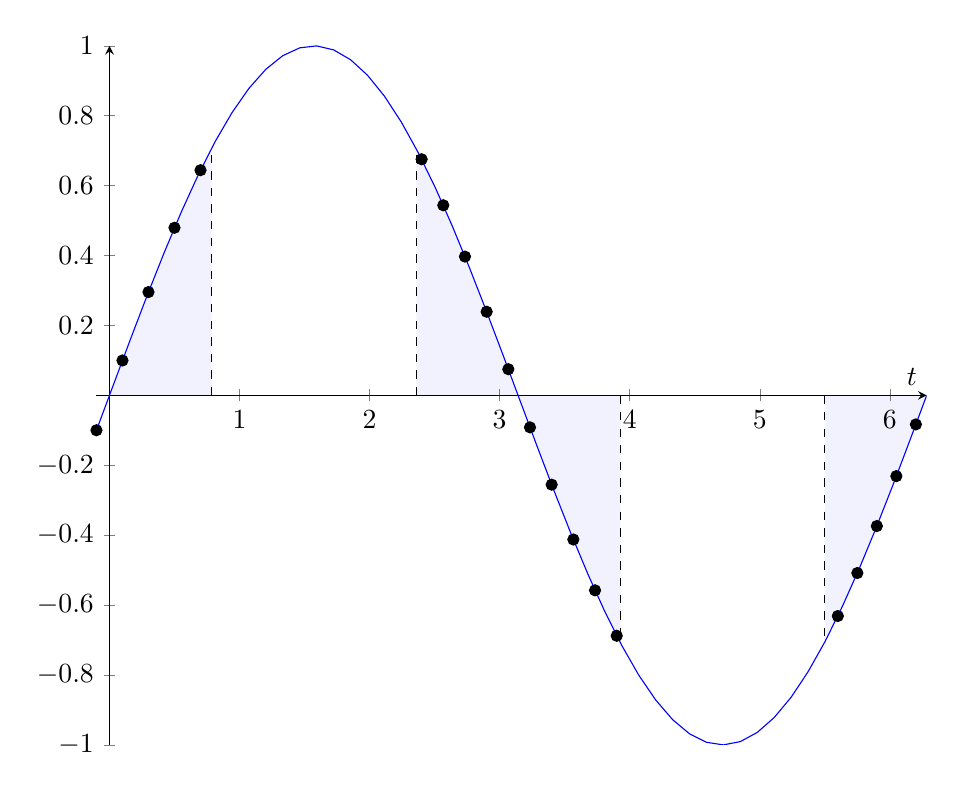
\begin{tikzpicture}
	\begin{axis}[axis lines=center, xlabel=$t$, domain=-.5:2*pi, legend pos=outer north east, width=\linewidth,
	scatter/use mapped color={draw=black, fill=black}
	]
	\addplot[color=blue, name path=signal, domain=-.1:2*pi,samples=50] {sin(deg(x))};
	\draw[dashed] (axis cs:.785,0) -- (axis cs:.785,{sin(deg(.785))});
	\draw[dashed] (axis cs:2.36,0) -- (axis cs:2.36,{sin(deg(2.36))});
	\draw[dashed] (axis cs:3.93,0) -- (axis cs:3.93,{sin(deg(3.93))});
	\draw[dashed] (axis cs:5.5,0) -- (axis cs:5.5,{sin(deg(5.5))});
	\path[name path=axis] (axis cs:0,0) -- (axis cs:2*pi,0);
	\addplot[fill=blue, opacity=.05] fill between [of=signal and axis, soft clip={domain=0:.785}];
	\addplot[fill=blue, opacity=.05] fill between [of=signal and axis, soft clip={domain=2.36:3.93}];
	\addplot[fill=blue, opacity=.05] fill between [of=signal and axis, soft clip={domain=5.5:2*pi}];
	\addplot [scatter, only marks, domain=-.1:.7, samples=5] {sin(deg(x))};
	\addplot [scatter, only marks, domain=2.4:3.9, samples=10, mark=*] {sin(deg(x))};
	\addplot [scatter, only marks, domain=5.6:6.2, samples=5, mark=*] {sin(deg(x))};
	\end{axis}     
	\end{tikzpicture}
	
	\end{minipage}%
	\begin{minipage}{.4\linewidth}
	\caption{Частотно-модулированная выборка: измерения делаются только в максимально информативных точках,
		находящихся в окрестностях узлов сигнала\label{fig:modulated_sampling}}
	\end{minipage}
\end{figure}

Был сделан вывод о нецелесообразности использования модулированной схемы выборки. Она даёт только
малый выигрыш (40\%) по сравнению с немодулированной схемой, \emph{даже если} не учитывать вариацию 
анализирующей способности детектора. Учитывая, что максимальная скорость изменения соответствует
окрестности продольной ориентации вектора поляризации пучка, в которой анализирующая способность 
детектора минимальна, эффективность использования модулированной схемы ещё меньше.

Также важно отметить отсутствие прямой зависимости между частотой $\omega$ измеряемого сигнала, 
и стандартным отклонением оценки частоты $\sigma_{\hat\omega}$. То есть, нет принципиальной разницы
измеряется ли частота в 1 или 100~рад/сек. Это обстоятельство важно для методов детектирования ЭДМ, 
основанных на измерении частоты прецессии спина: благодаря ему, строго говоря, 
отсутствует необходимость подавлять МДМ-прецессию, связанную с неидеальностями 
оптической структуры ускорителя.

Также была оценена эффективная длительность измерительного цикла, 
исходя из времени жизни поляризации пучка  $\tau_d$ (опеределяемого как период времени, 
за который полярищация пучка уменьшается в $e$ раз). Очевидно, что когда пучок полностью деполяризуется, 
невозможно получать информацию о скорости вращения его поляризации; т.е. 
существует принципиальное ограничение на полное количество информации (обозначим её $\mathrm{FI_{tot}}$) 
о частоте прецессии спина, которое можно получить за один цикл измерений.
В таблице~\ref{tbl:FItot} отражено количество выбранной (относительно $\mathrm{FI_{tot}}$) информации 
о частоте прецессии спина как функция длительности цикла, а также соответствующее ему отношение
сигнал/шум. Исходя из данных таблицы, полезная длительность измерительного цикла 
ограничена тремя постоянными времени деполяризации.

Результаты численного моделирования~\cite{Aksentev:Stats} показывают 
возможность достичь точности оценки частоты прецессии спина 
на уровне ${8\cdot 10^{-7}}$~рад/сек за один измерительный цикл при постоянной времени деполяризации 
1 000~сек, частоте измерения поляризации 375~Гц, и начальной ошибке измерения поляризации 3\%. 
При 70\%  годовой временной загрузке ускорителя это позволяет выйти на уровень 
${5\cdot 10^{-9}}$~рад/сек стандартного отклонения среднего значения оценки частоты. 
Такая точность достаточна для получения оценки ЭДМ на уровне $10^{-29}~e\cdot$см.

\begin{table}[H]\captionsetup{width=.75\linewidth}
	\caption{Количество выбранной информации (в долях от потенциального максимума), 
		в зависимости от длительности измерительного цикла, 
		и соответствующее ему отношение сигнал/шум.\label{tbl:FItot}}
	\centering
	\begin{tabular}{rrr}
		\toprule
		Инфо. (\%$\mathrm{FI_{tot}}$) & Длительность ($\times\tau_d$) & Сигнал/шум  \\
		\midrule
		95            & 3.0                     & 0.4         \\
		90            & 2.3                     & 1.1         \\
		70            & 1.2                     & 5.5         \\
		50            & 0.7                     & 11.7        \\
		\bottomrule
	\end{tabular}
\end{table}

В \textbf{Главе 4} описаны наиболее значимые (для данной работы) технологии, 
разработанные в рамках исследований, проведённых на синхротроне COSY (Рис.~\ref{fig:COSY_Ring}), 
а также описаны результаты процедуры оптимизации времени когерентности спина (spin coherence time, SCT) 
при помощи семейств секступолей, установленных на COSY
(параметры COSY  представлены в Таблице~\ref{tbl:COSY-studies}).

\begin{figure}[H]\centering
	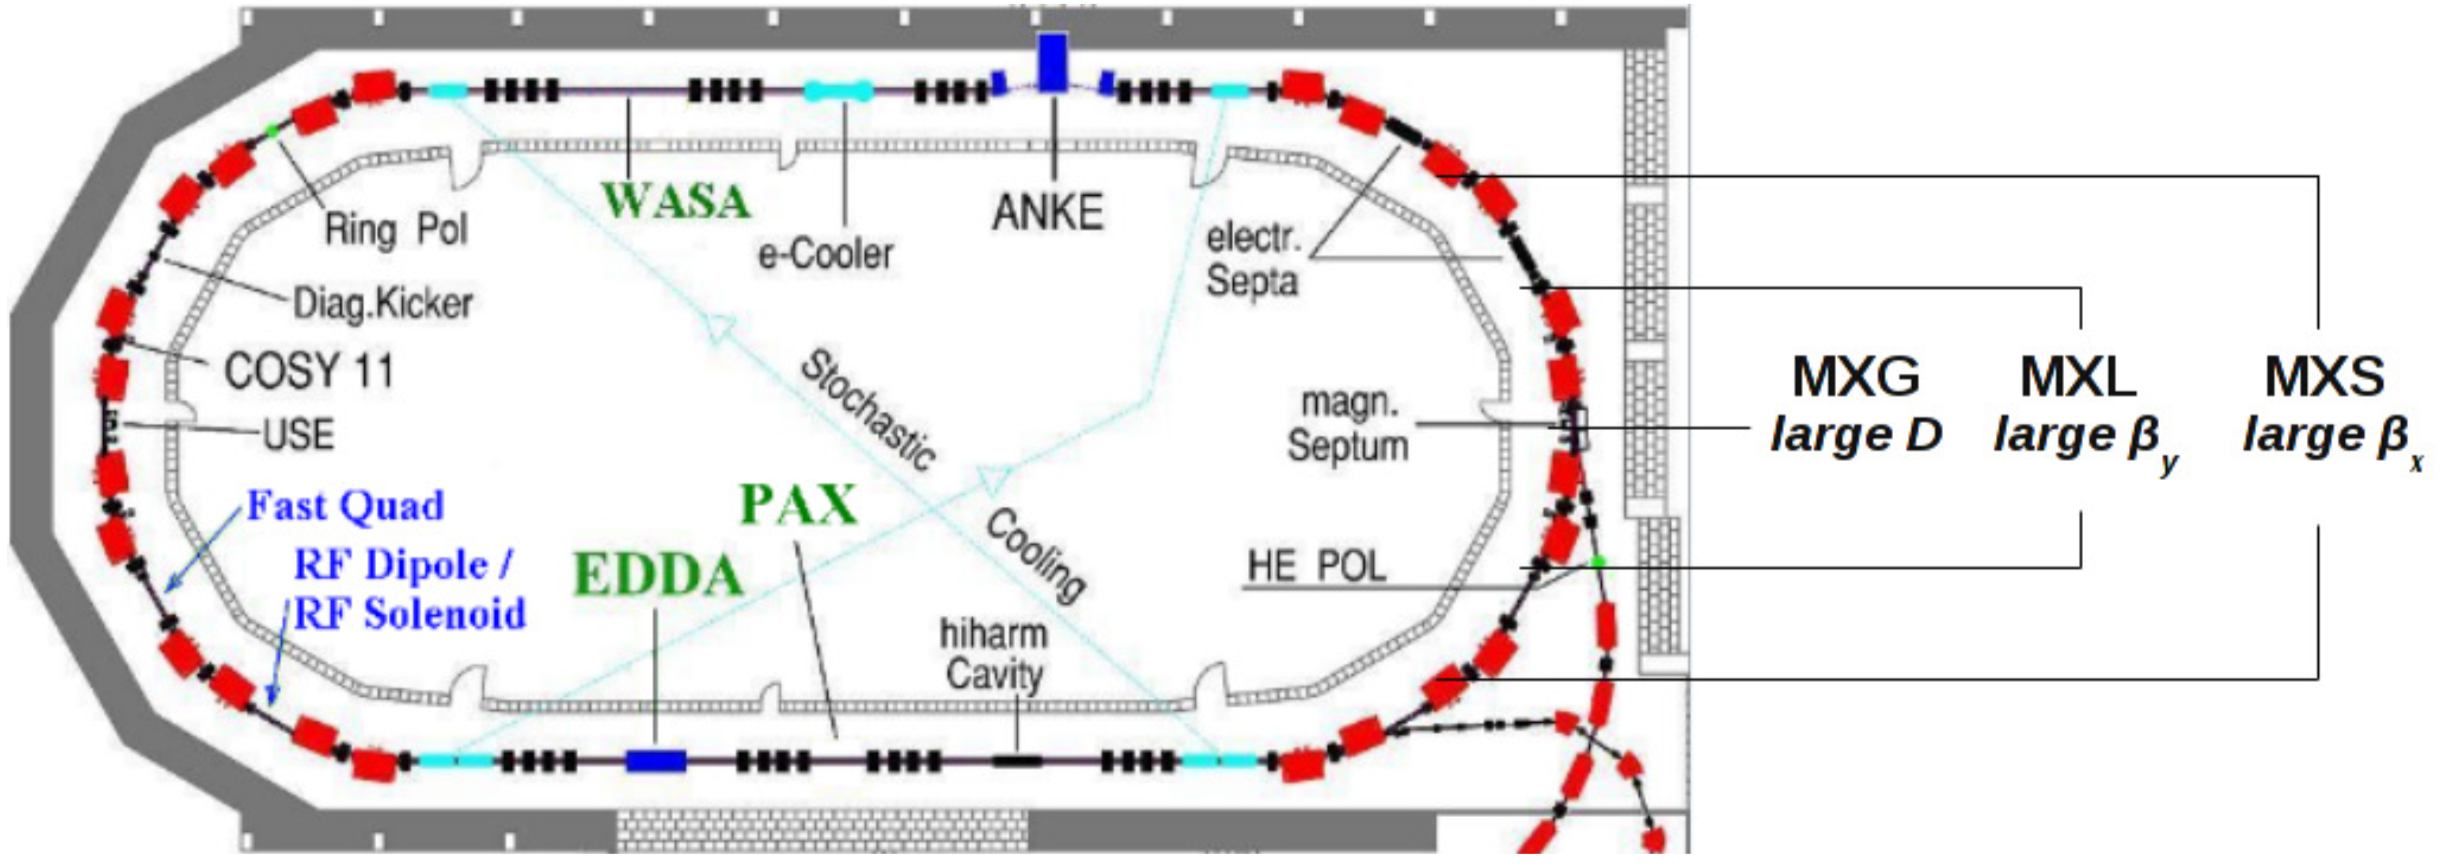
\includegraphics[width=\linewidth]{images/chapter4/COSY-sextupoles}
	\caption{Кольцо COSY с отмеченными положениями секступолей для контроля времени когерентности спина~\cite{Guidoboni:STORI14}\label{fig:COSY_Ring}}
\end{figure}


\begin{table}[H]\centering\captionsetup{width=.95\linewidth}
	\caption{Рабочие параметры COSY, использованные в проводимых исследованиях\label{tbl:COSY-studies}}
	\begin{tabular}{lll}
		\toprule
		Параметр & Величина & Размерность \\
		\midrule
		Длина окружности COSY& 183 & м\\
		Импульс дейтрона & 970 & МэВ/с \\
		$\beta$ / $\gamma$ & 0.459 / 1.126 & \\
		Аномальный магнитный момент G& -0.143& \\
		Частота оборота пучка $f_{\mathrm{rev}}$& 752543& Гц\\
		Длительность измерительного цикла& 100--1500& сек\\
		Число частиц в пучке & $\approx 10^9$& \\
		\bottomrule
	\end{tabular}
\end{table}

Рассмотренные технологии:
\begin{enumerate}[(1)]
	\item высокоточное измерение спин-тюна (с точностью до $10^{-10}$ в измерительном цикле 100~секунд);
	\item юстировка квадруполей при помощи пучка (Beam Based Alignment~\cite{Wagner:BBA2018});
	\item оптимизация времени когерентности спина~\cite{COSY:SCT:IPAC15, Guidoboni:STORI14}.
\end{enumerate} 

Отдельно стоит отметить наблюдение явления изменения SCT (см. Рис.~\ref{fig:April2019:Polarization}) 
при длительном измерении поляризации разрушающими методами, связаного с переходом 
от внешней (ореол) к внутренней (ядру) частям пучка. 
Наблюдение этого явления косвенно подтверждает теорию спин-декогеренции, изложенную в данной работе.

\begin{figure}[H]\centering
	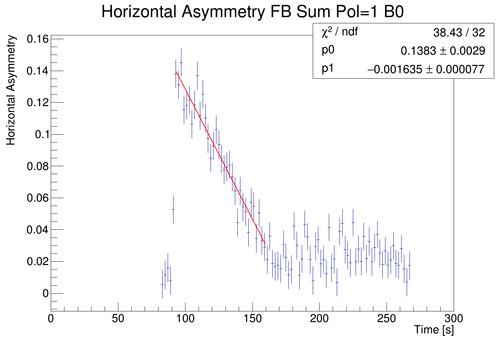
\includegraphics[height=.3\paperheight]{images/chapter4/SCT-April-2019/11th_20-20}
\caption{Результаты измерения горизонтальной поляризации во время оптимизации времени когерентности спина при подготовке к эксперименту по поиску аксионов в апреле 2019 года\label{fig:April2019:Polarization}}
\end{figure}


В \underline{\textbf{заключении}} приведены основные результаты работы, которые заключаются в следующем:
%% Согласно ГОСТ Р 7.0.11-2011:
%% 5.3.3 В заключении диссертации излагают итоги выполненного исследования, рекомендации, перспективы дальнейшей разработки темы.
%% 9.2.3 В заключении автореферата диссертации излагают итоги данного исследования, рекомендации и перспективы дальнейшей разработки темы.

\begin{enumerate}
	\item Разработан метод измерения электрического дипольного момента дейтрона, 
	основанный исключительно на измерении частоты прецессии спина.
	\item Предложен принцип построения магнитооптической структуры кольца-накопителя, 
	ориентированного на поиск электрического дипольного момента дейтрона.
	\item Получены результаты исследования спин-декогеренции пучка дейтронов в окрестности 
	состояния ``замороженного спина'', а также метод подавления спин-декогеренции, основанный на использовании нелинейных элементов.
	\item Исследованы эффекты различного рода несовершенств элементов накопительного кольца 
	на спин-орбитальную динамику пучка.
	\item Проведено численное моделирование матода калибровки нормализованной частоты прецессии спина 
	при попеременной смене полярности ведущего поля накопительного кольца.
	\item Исследованы систематические ошибки в различных предложениях по проведению эксперимента 
	по поиску электрического дипольного момента; проведён сравнительный анализ этих предлодений 
	с методом Frequency Domain.
	\item Проведена оценка статистических свойств Frequency Domain метода измерения 
	электрического дипольного момента в накопительном кольце.
\end{enumerate}
%\begin{enumerate}
%  \item Были изучены эффекты спиновой динамики, составляющие систематические ошибки эксперимента по поиску
%  электрического дипольного момента частицы методом замороженного спина в накопительном кольце, как то:
%  \begin{itemize}
%  	\item возмущения спиновой динамики вызванные бетатронным движением частицы;
%  	\item декогеренция спинов частиц пучка;
%  	\item МДМ прецессия спина, вызванная неидеальностями ускорителя.
%  \end{itemize}
%  \item Для каждого из эффектов, было описано средство борьбы, и проведено численное моделирование,
%  подтверждающее его эффективность.
%  \item Были сформулированы:
%  \begin{itemize}
%  	\item понятия методов пространственной и временной областей;
%  	\item понятие двумерно-замороженного спина;
%  	\item необходимые условия успешного измерения ЭДМ в накопительном кольце;
%  	\item метод Frequency Domain, удовлетворяющий всем сформулированным условиям.
%  \end{itemize}
%  \item Описаны структуры накопительных колец с непрерывно- и квази-замороженным спином.
%\end{enumerate}


\ifdefmacro{\microtypesetup}{\microtypesetup{protrusion=false}}{} % не рекомендуется применять пакет микротипографики к автоматически генерируемому списку литературы
\ifnumequal{\value{bibliosel}}{0}{% Встроенная реализация с загрузкой файла через движок bibtex8
  \renewcommand{\bibname}{\large \authorbibtitle}
  \nocite{*}
  \insertbiblioauthor           % Подключаем Bib-базы
  %\insertbiblioother   % !!! bibtex не умеет работать с несколькими библиографиями !!!
}{% Реализация пакетом biblatex через движок biber
  \ifnumgreater{\value{usefootcite}}{0}{
%  \nocite{*} % Невидимая цитата всех работ, позволит вывести все работы автора
  \insertbiblioauthorcited      % Вывод процитированных в автореферате работ автора
  }{
  \insertbiblioauthor           % Вывод всех работ автора
%  \insertbiblioauthorgrouped    % Вывод всех работ автора, сгруппированных по источникам
%  \insertbiblioauthorimportant  % Вывод наиболее значимых работ автора (определяется в файле characteristic во второй section)
  \insertbiblioother            % Вывод списка литературы, на которую ссылались в тексте автореферата
  }
}
\ifdefmacro{\microtypesetup}{\microtypesetup{protrusion=true}}{}
